\begin{frame}
	\frametitle{22 августа, день 5}
	\framesubtitle{м.н.~--- д.р. Джалпаккол~--- д.р. Кичкинекол Джалпаккольский} % Optional subtitle
	\begin{columns}[c] % The "c" option specifies centered vertical alignment while the "t" option is used for top vertical alignment
		\begin{column}{0.45\textwidth} % Left column width
			\begin{itemize}
				\item Прохождение каменного лабиринта
				\item Гроза
			\end{itemize}
			
		\end{column}
		\begin{column}{0.5\textwidth} % Right column width
			\centering
			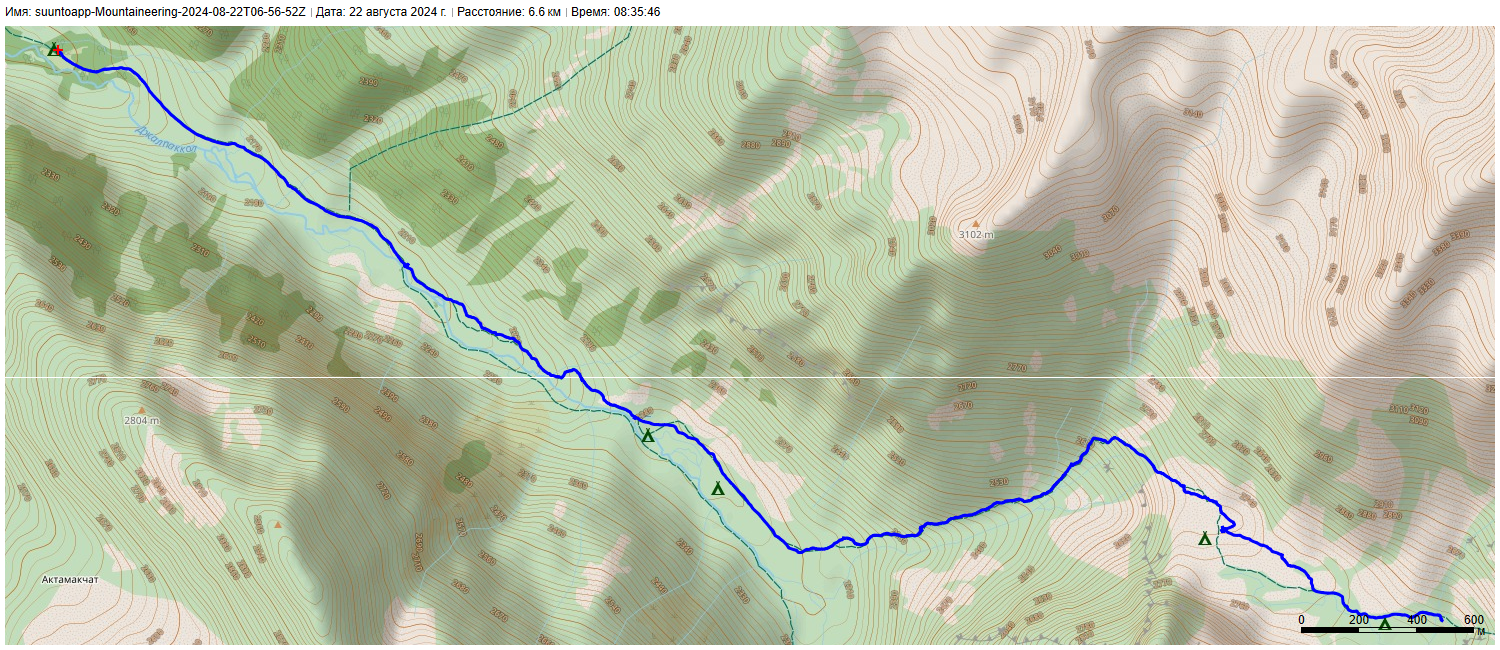
\includegraphics[width=\linewidth]{../pics/mini_maps/22}
		\end{column}
	\end{columns}
\end{frame}